%\documentclass[11pt, oneside]{article}   	
%\usepackage{geometry}    
%\geometry{letterpaper}                 		
\input preamble.tex
\newcommand{\ig}[2][width=4in]{\includegraphics[#1]{#2}}    		
\usepackage{graphicx}					
\usepackage{amssymb}
\usepackage{pgfplotstable}
\usepackage{float}
\usepackage{caption}
\captionsetup[table]{justification=justified,singlelinecheck=false, position=bottom}
\begin{document}

\header {\today}							
\title{Muon Lifetime}
\author{Ekta Patel \& Brandon Booth-Dunbar}

\section{Abstract}
%Ekta
\begin{em} Positively charged muons reach the Earth via cosmic ray showers.When they decay, the muons break down into a positron, an electron neutrino and a muon neutrino.The goal of the experiment is to measure the lifetime of the muon by detecting and stopping a positive muon in an aluminum slab and then consequently detected the positron that it leaves behind when it decays.The distribution of the difference in detection times can be used to determine the muon lifetime.
\end{em}

\section{Theory}
%Brandon

\section{Experimental Methods}
%Ekta, but I (Brandon)  will make the figures
\subsection{Apparatus}
\indent  \indent As a positively charged muon reaches the Earth and hits the scintillation detector, a small flash of light is observed due to the plastic sheet of the scintillator. The photomultiplier then changes the flash of light into a pulse of electrons which then travels to an amplifier/discriminator that filters away the noise from the detector in addition to strengthening the incoming pulse of electrons. The amplifier/discriminator then feeds the output pulse into the coincidence circuit to ensure that only the positrons and muon electrons are detected. 
\newline \indent We want to start a clock when a positive muon is detected in the aluminum slab and stop the clock when the positron is detected from the muon decay. The distribution of a very large number of delay times, created by the `start' and `stop' of the detections, will be used to determine the lifetime of the muon. 
\newline \indent In our setup, we have three photomultipliers($A, B, C$), two of which will trap the muon long enough for it to decay and a third that will help in the detection of the positron. We use the $A$ and $B$ photomultipliers to detect and trap the muon. When $A$ and $B$ are triggered, but not C, the clock will start to count until either $B$ or $C$ is triggered again by the positron and stops the clock. We do not want all three photomultipliers to be triggered when the muon is detected because the time delay will be irrelevant since the clock will start and stop almost instantaneously. We need the muon to be trapped by two photomultipliers and the resulting positron to be detected by one of the photomultipliers. Therefore, the start and stops of the clock correspond to:
\begin{equation} start: \textbf A\;and\; \textbf B \end{equation}
\begin{equation} stop: \textbf B\; or\; \textbf C \end{equation}
Though we choose to setup our apparatus in this way, there is also another possibility in which the $A$ and $B$ photomultipliers are used to detect the muon but then only $B$ exclusively or C detect the positron ($B$ XOR $C$). This setup guarantees that the clock would only be stopped if either $B$ or $C$ were activated, but not both since the positron only travels either up or down through the apparatus as the muon decays. However, we do not choose to set up our experiment that way because it is not likely that another muon will be detected faster than in the time scales that we are observing. Since the muon realistically only takes about 2 $\mu$s to decay, a false trigger of photomultiplier $B$ would have to take place in that much time or less. The muon sea level flux is only 1 /cm$^2$/minute or about one muon every 6x10$^7\mu$s.%Add what the average counts per second for B was and discuss the rate% 
\newline \indent The Time-to-Amplitude Converter converts the times between each `start' and `stop'  to voltages. These voltages are then recorded by the Multi-Channel Analyzer which uses the computer to bin the data into a histogram based on the strengths of voltages which correspond to the lengths of times taken for each detected muon to decay. It is important to remember that the muon flux at sea level is only 1 /cm$^2$/minute, so we will need to take data sets that stretch over several days to a few weeks to get a good distribution of delay times. 
\newline \indent 
\begin{figure}[H]
\begin{center}
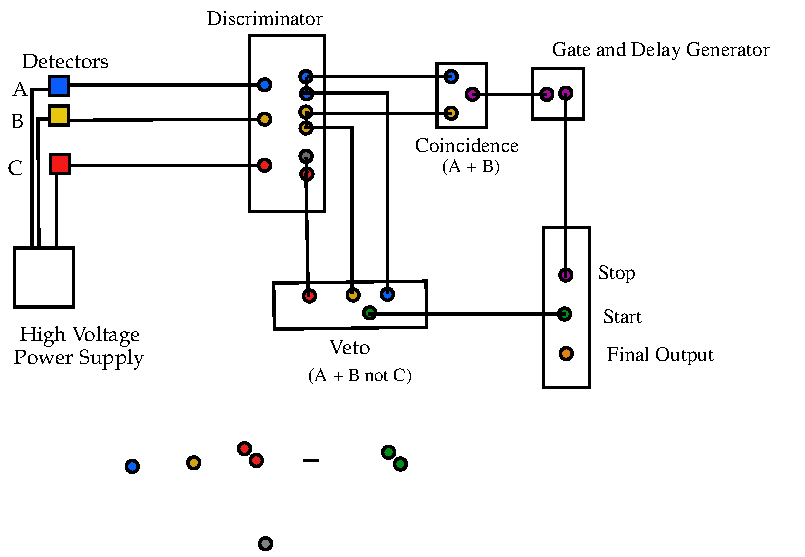
\includegraphics[width=4 in]{ML-figure1.pdf}
\caption{Bitches be figurin'}
\end{center}
\end{figure}

\subsection{Procedure}
%get voltage values for each of the detectors


\section{Results \& Discussion}
%Brandon

\section{Conclusion}
%Ekta

\begin{thebibliography}{99}
%\bibitem{}
\end{thebibliography}

\newpage \LARGE{Appendix}

\end{document}  
